% thesis.tex
%
% This file is root file for an example thesis written using the
% IIT Bombay LaTeX Style file.
% Created by Amey Karkare (21 June 2007)
%
% It is provided without warranty on an AS IS basis.

%=====================================================================
% Read: http://www.cse.iitb.ac.in/karkare/iitbthesis/
%    FAQ.txt     for frequently asked quetions
%    Changes.txt for changes
%    README      for more information
%=====================================================================

%=====================================================================
% DOCUMENT STYLE
%=====================================================================
% IITB PhD Thesis format default settings are:
%   12pt, one-sided printing on a4 size paper
\documentclass[openright,twoside]{iitkthesis}
% For two-sided printing, with Chapter starting on odd-numbered pages,
% use the following line instead:
%%\documentclass[openright,twoside]{iitbthesis}

%=====================================================================
% OPTIONAL PACKAGES
%=====================================================================
% To include optional packages, use the \usepackage command.
% For e.g., The package epsfig is used to bring in the Encapsulated
%    PostScript figures into the document.
%    The package times is used to change the fonts to Times Roman;
%=====================================================================

%=====================================================================
%  Single counter for theorems and theorem-like environments:
%=====================================================================
\newtheorem{theorem}{Theorem}[chapter]
\newtheorem{assertion}[theorem]{Assertion}
\newtheorem{claim}[theorem]{Claim}
\newtheorem{conjecture}[theorem]{Conjecture}
\newtheorem{corollary}[theorem]{Corollary}
\newtheorem{definition}[theorem]{Definition}
\newtheorem{example}[theorem]{Example}
\newtheorem{figger}[theorem]{Figure}
\newtheorem{lemma}[theorem]{Lemma}
\newtheorem{prop}[theorem]{Proposition}
\newtheorem{remark}[theorem]{Remark}

\usepackage{minted}
\usemintedstyle{bw}

\usepackage{fontspec}
\setmonofont[Scale=0.85]{DejaVu Sans Mono}

\usepackage[sorting=none, maxbibnames=99, minbibnames=99, backend=biber]{biblatex}
\bibliography{citations}
\usepackage{amsmath}
\usepackage{lipsum}
\usepackage{float}
\usepackage[hidelinks]{hyperref}
\usepackage{microtype}
\usepackage[font=small,labelfont=bf]{caption}
\usepackage{fancyref}
\usepackage{color,soul} % for highlights
\usepackage{enumerate}
\usepackage{tabularx}

\setlength{\headheight}{15pt}

\expandafter\def\csname PY@tok@err\endcsname{}

\floatstyle{ruled}
\newfloat{program}{thp}{lop}
\floatname{program}{Figure}

\numberwithin{program}{chapter}

\BeforeBeginEnvironment{program}{\begin{singlespace}}
\AfterEndEnvironment{program}{\end{singlespace}}

%=====================================================================
% End of Preamble, start of document
%

\begin{document}

%=====================================================================
% Include the prelude for Title page, abstract, table of contents, etc
% You need to modify it to contain your details
% prelude.tex
%   - titlepage
%   - dedication (optional)
%   - approval sheet
%   - course certificate
%   - table of contents, list of tables and list of figures
%   - nomenclature
%   - abstract
%============================================================================


\clearpage\pagenumbering{roman}  % This makes the page numbers Roman (i, ii, etc)



% TITLE PAGE
%   - define \title{} \author{} \date{}
\title{Bloc: Library for handling large binary objects in Haskell}
\author{Anshu Avinash}
\date{June, 2015}

%  - Roll number, required for title page, approval sheet, and
%    certificate of course work
\rollnum{10327122}

%   - The default degree is ``Doctor of Philosophy''
%     (unless the document style msthesis is specified
%      and then the default degree is ``Master of Science'')
%     Degree can be changed using the command \iitbdegree{}
\iitbdegree{Master of Technology}

%   - The default report type is preliminary report.
%      * for a PhD thesis, specify \thesis
\thesis
%      * for a M.Tech./M.Phil./M.Des./M.S. dissertation, specify \dissertation
%\dissertation
%      * for a DIIT/B.Tech./M.Sc.project report, specify \project
%\project
%      * for any other type, use  \reporttype{}
%\reporttype{ReportType}

%   - The default department is ``Unknown Department''
%     The department can be changed using the command \department{}
\department{Computer Science \& Engineering}

%    - Set the guide's name
\setguide{Prof Piyush Kurur}
\setguidedept{Department of Computer Science \& Engineering}

%   - once the above are defined, use \maketitle to generate the titlepage
\maketitle

%--------------------------------------------------------------------%
% CERTIFICATE
%     The first page after the title page.
\makecertificate

%--------------------------------------------------------------------%
% COPYRIGHT PAGE
%   - To include a copyright page use \copyrightpage
% \copyrightpage

%--------------------------------------------------------------------%
% ABSTRACT
\begin{abstract}
  In this thesis, we describe a library for handling large binary objects (blob) written in Haskell - a purely-functional programming language. We use the idea of storing each blob as a separate file. We also try to make all the operations on a blob to be safe under concurrent access without using any locks. We leverage many features offered by Haskell like modularity and strong type system.

\end{abstract}

%--------------------------------------------------------------------%
% DEDICATION
%   Dedications, if any.
\begin{dedication}
Placeholder
\end{dedication}

% Acknowledgements
\begin{acknowledgments}
Placeholder
\end{acknowledgments}

%--------------------------------------------------------------------%
% CONTENTS, TABLES, FIGURES
\tableofcontents
\listoftables

\cleardoublepage
\listoffigures

\listof{program}{List of Programs}
\addcontentsline{toc}{chapter}{List of Programs}

\cleardoublepage\pagenumbering{arabic} % Make the page numbers Arabic (1, 2, etc)


%=====================================================================
% Include the technical part of the report
%% \include{chap_intro}             % Chapter 1: Introduction
%% \include{chap_others}            % Other chapters as required
%% \include{chap_conclusions}       % Finally the summary & conclusions

%=====================================================================
% APPENDIX
%  Appendices, if any, must precede the cited literatures.
%  Appendices shall be numbered in Roman Capitals (e.g. Appendix IV)

%% \appendix
%% \include{appendix_something}

%=====================================================================
% PUBLICATIONS
%  publications if any may be listed after the literature cited.
%% \include{mypubs}

%=====================================================================
% ACKNOWLEDGMENTS
%   This is the last item in the thesis. It should be signed by
%   author, with date.

\chapter{Introduction}
\label{chap:intro}

Most of the web applications today require to store some kind of data persistently. For a web application that handles student management - the data can be name, date of birth, photograph and other information about students. These web applications use one of the \textit{databases} to store their data. Database refers to a collection of information that exists overs a long period and a Database Management System (DBMS) is a tool for creating and managing large amount of data efficiently.

Early database management systems evolved from file systems. These database systems used tree-based and the graph-based models for describing the structure of the information in a database. Edgar F. Codd in his seminal paper~\cite{codd1970relational} proposed that database systems should present the user with a view of data organized as tables called relations. This paper set the foundation for popular relational databases like MySQL and PostgreSQL.

Many of the web applications do not require the complex querying and management functionality offered by a Relational Database Management System (RDBMS). This among other reasons gave rise to several NoSQL (Not only SQL) databases. NoSQL databases can be classified based on the data models used by them. Amazon's Dynamo~\cite{decandia2007dynamo} is a key-value store in which records are stored and retrieved using a key that uniquely identifies the record.
MongoDB~\cite{chodorow2013mongodb} on the other hand is a document-oriented database and is designed for managing semi-structured data. These NoSQL databases offer an important benefit of scalability and availability by sacrificing strong consistency guarantees offered by RDBMS.

Today's web applications also work with large files like images, music, videos etc. Size of these files can vary from few MBs to tens of GBs. The application developer can decide to store these files directly into the one of the databases mentioned above or store it as a file and save the filename in the database. This large binary data is usually called a blob (\textbf{B}inary \textbf{L}arge \textbf{OB}ject).

In this thesis, we provide a library written in Haskell - a purely functional programming language, for handling blobs. The library provides methods for incremental writing, incremental reading and garbage collection of deleted blobs.

Concurrency plays an important part in building scalable and fault tolerant web applications. However, building concurrent systems usually requires working with locks and may result into issues like deadlock and starvation. By making use of the atomic guarantees provided by the file system on certain file operations, we provide lock free concurrent access to blobs.

The name of our library ``Bloc'' stands for \textbf{B}inary \textbf{L}arge \textbf{O}bjects with \textbf{C}oncurrency, since it deals with blobs and provides support for concurrent operations.

\section{Organization of the thesis}
Chapter 2 discusses the approach of storing large files in databases. It also provides a background for this thesis work. In Chapter 3, we give a brief introduction to functional programming. Chapter 4 describes our design and implementation. We conclude and present the future work in Chapter 5.

\chapter{Design and Implementation}
\label{chap:design}

Our design is inspired from the maildir format~\cite{bernstein1995using}. The maildir format stores each message in a separate file with a unique name. The mail user agent (MUA) does not have to worry about partially delivered mail: each message is safely written to disk in the \textit{tmp} subdirectory before it is moved to \textit{new}. When a mail user agent process finds message in the \textit{new} subdirectory, it moves them to \textit{cur}.

Similar to maildir, we also store all large objects in separate files. All the large objects of a database are stored under a single directory which we also call a ``BlobStore''.
The BlobStore contains three subdirectories: \textit{tmp}, \textit{curr} and \textit{old}. We will discuss purpose of these directories later in this chapter.

\section{Initializing the BlobStore}
Before starting to create blobs inside a directory, we ensure that the \textit{tmp} and \textit{curr} subdirectories have already been created. We provide a method \texttt{initBlobStore} which takes the path of a directory which is to be used as BlobStore as argument and does the initialization for us.
BlobStore is defined as a newtype. We don't expose the constructor for BlobStore, so the only way to get a BlobStore is by using the \texttt{initBlobStore} method.

\begin{program}
  \caption{Definition of BlobStore}
  \label{prog:defblobstore}
  \inputminted{haskell}{hs/blobstore.hs}
\end{program}

\section{Creating a Blob}
We provide a method called \texttt{createBlob} for creating a new blob. It takes a BlobStore as a parameter and returns a WriteContext.

\begin{program}
  \caption{Definition of WriteContext}
  \label{prog:defwritecontext}
  \inputminted{haskell}{hs/writecontext.hs}
\end{program}

WriteContext contains the file handle of just created blob, a TempLocation and a hashCtx. TempLocation stores the base directory and the filename of just created blob. The hashCtx is used to store the SHA-512 hash of the contents that has been written to the blob.

All the new blobs are created in the \textit{tmp} folder. We use Version 4 UUID~\cite{leach2005universally} to give unique names to the newly created blobs.

\section{Writing to a Blob}
We only allow to add new data at the end of a given blob. We provide \texttt{writePartial} method for this. \texttt{writePartial} takes a blob and a WriteContext as arguments and appends the given blob to the WriteContext's blob.
Once all the data has been written to the blob, \texttt{finalizeWrite} is called. \texttt{finalizeWrite} takes a WriteContext as argument and moves the blob from \textit{tmp} folder to \textit{curr} folder. We also rename the file to SHA-512 hash of its contents.
\texttt{finalizeWrite} returns a BlobId. This BlobId contains the location of the blob.
No more updates to the blob are possible after calling \texttt{finalizeWrite}.

\begin{program}
  \caption{Definition of BlobId}
  \label{prog:defblobid}
  \inputminted{haskell}{hs/blobid.hs}
\end{program}

\begin{figure}[hbt]
  \caption{Directory structure of a BlobStore}
  \label{fig:blobstore-dirstructure}
  \dirtree{%
    .1 blobstore.
    .2 tmp.
    .3 f66affb7-ad10-4583-8986-c4a6892d0120.
    .2 curr.
    .3 sha512-a75ebf9a0f109288d3eae1ecbfd89....
  }
\end{figure}

\section{Reading from Blob}
Reading is also sequential. First the \texttt{initRead} method is called which takes a BlobId as argument and returns a ReadContext. ReadContext also contains the file handle of the blob which is opened in read mode.

\begin{program}
  \caption{Definition of ReadContext}
  \label{fig:defreadcontext}
  \inputminted{haskell}{hs/readcontext.hs}
\end{program}

\texttt{readPartial} takes a ReadContext and number of bytes as input and returns those number of bytes from the blob.
While reading from a blob, you can skip ahead using the method \texttt{skipBytes}. \texttt{skipBytes} takes a ReadContext and number of bytes, \textit{b} as input and skips \textit{b} bytes ahead in the ReadContext.

\begin{table}[hbt]
\caption{Interface for operations on blob}
\label{tab:interface-blob}
\begin{center}
  \begin{tabularx}{0.91\textwidth}{lX}
    \hline\noalign{\smallskip}
    Methods & Purpose \\
    \noalign{\smallskip}
    \hline
    \noalign{\smallskip}
    \texttt{initBlobStore} & Initializes given directory to be used as a BlobStore \\
    \texttt{createBlob} & Creates a blob in the given BlobStore\\
    \texttt{writePartial} & Takes a blob and appends it to the end of the blob given in the argument\\
    \texttt{finalizeWrite} & Takes a WriteContext as input and returns a BlobId \\
    \texttt{initRead} & Takes a BlobId as input and returns a ReadContext \\
    \texttt{readPartial} & Reads a given number of bytes from a Blob \\
    \texttt{skipBytes} & Skips ahead a given number of bytes in a Blob \\
    \texttt{finalizeRead} & Completes the read \\
    \hline
  \end{tabularx}
\end{center}
\end{table}

\begin{figure}
  \caption{Order of operations on Blob}
  \label{fig:blob-operations-order}
  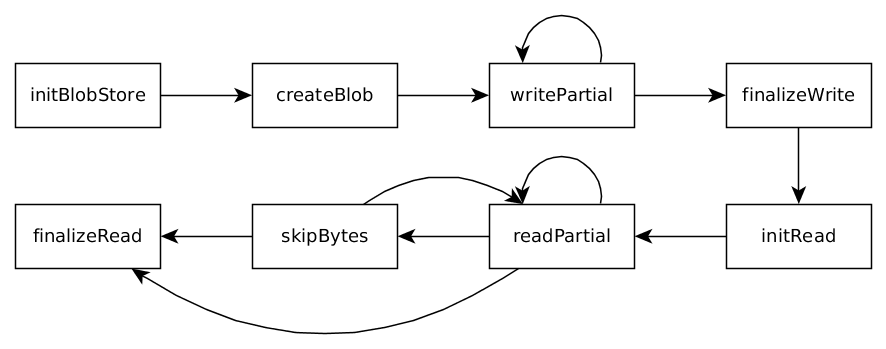
\includegraphics[scale=0.5]{figures/blob_operations_order.png}
\end{figure}

\section{Garbage Collection}
It is quite likely that the same blob would be shared by multiple ``values'' in the database. For a relational database these values are rows in a table, while for a document-oriented database, these values are documents.
Hence, we provide an interface for garbage collecting the deleted blobs.

\subsection{Starting the Garbage Collection}
The \texttt{startGC} method takes a BlobStore as argument and starts garbage collection (GC) for that BlobStore.
\texttt{startGC} does two things: It first renames the \textit{curr} folder to \textit{old} and then creates an empty \textit{curr} folder.
Once a GC has started you can not start another GC on the same BlobStore until the first one finishes - doing so will throw an error. Also, note that creation of new blobs and reading the old blobs can happen concurrently with the GC.

\begin{figure}[hbt]
  \caption{Directory structure of a BlobStore during GC}
  \label{fig:blobstore-dirstructure-gc}
  \dirtree{%
    .1 blobstore.
    .2 tmp.
    .3 1a4c5091-1295-4c9c-b8d3-8e6123a51b41.
    .2 old.
    .3 sha512-9b71d224bd62f3785d96d46ad3ea3....
    .2 curr.
    .3 sha512-11853df40f4b2b919d3815f64792e....
  }
\end{figure}

\subsection{Marking a blob as accessible}
Once a blob is marked as not deleted using the method \texttt{markBlobAsAccessible}, we move it from the \textit{old} folder to the \textit{curr} folder. This ensures that the blob does not get deleted at the end of the GC.

\subsection{End Garbage collection}
This step involves removal of all the blobs which are not accessible. The \texttt{endGC} method takes a BlobStore as argument and delete the \textit{old} subdirectory along with its contents.

\begin{table}[hbt]
\caption{Interface for garbage collection}
\label{tab:interface-gc}
\begin{center}
  \begin{tabularx}{0.91\textwidth}{lX}
    \hline\noalign{\smallskip}
    Methods & Purpose \\
    \noalign{\smallskip}
    \hline
    \noalign{\smallskip}
    \texttt{startGC} & Starts garbage collection for the given BlobStore\\
    \texttt{markBlobAsAccessible} & Marks the given blob as accessible\\
    \texttt{endGC} & Ends the garbage collection by removing all the unaccessible blobs\\
    \hline
  \end{tabularx}
\end{center}
\end{table}

\section{Concurrency}
In this section we will describe how the design described above allows concurrent access on blobs across processes.

\chapter{Implementation}
\label{chap:implementation}

\begin{singlespace}
\cleardoublepage
\phantomsection \label{listoffig}
\addcontentsline{toc}{chapter}{References}
\renewcommand\bibname{References}
\printbibliography
\nocite{*}
\end{singlespace}

\end{document}
